The main purpose of a calorimeter is to measure the energy of electrons, photons
and hadrons by mean of materials capable of completely absorb the energy of the
incoming particles transforming it in some measurable quantity. Calorimeters can
be classified in two categories, \emph{electromagnetic} (EM) and \emph{hadronic}
depending on the particle they are designed to detect. The EM calorimeters are
mainly used to detect photons and electrons while the task of hadronic
calorimeters is to identify hadrons. Both types of can be further divided into
\emph{sampling calorimeters} and \emph{homogeneous calorimeters}. Sampling
calorimeters alternates layers of a dense material used to absorb the energy of
incident particles (absorber) and an active material to collect the signal. The
interaction between the particles and the absorber produces a shower of
secondary particles with progressively degraded energy which is deposited in the
active material in form of charge or light that can be converted into
energy. Homogeneous calorimeters use only one material that serves both as an
absorber and an active material\cite{Calorimetry}.

The ATLAS calorimeter is a sampling calorimeter covering up the $|\eta| < 4.9$
region, an illustration of the system is shown in Figure~\ref{fig:calo}.
\begin{figure}[!h]
  \centering
    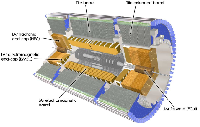
\includegraphics[width=.5\linewidth]{calorimeters}
    \caption{Cut-away view of the ATLAS calorimeter system.}
    \label{fig:calo}
\end{figure}
%%% Local Variables:
%%% mode: latex
%%% TeX-master: "../search_for_DM_LED_with_ATLAS"
%%% End:
